%
%  GL2PS, an OpenGL to PostScript Printing Library
%  Copyright (C) 1999-2011 C. Geuzaine
%
%  This program is free software; you can redistribute it and/or
%  modify it under the terms of either:
%
%  a) the GNU Library General Public License as published by the Free
%  Software Foundation, either version 2 of the License, or (at your
%  option) any later version; or
%
%  b) the GL2PS License as published by Christophe Geuzaine, either
%  version 2 of the License, or (at your option) any later version.
%
%  This program is distributed in the hope that it will be useful, but
%  WITHOUT ANY WARRANTY; without even the implied warranty of
%  MERCHANTABILITY or FITNESS FOR A PARTICULAR PURPOSE.  See either
%  the GNU Library General Public License or the GL2PS License for
%  more details.
%
%  You should have received a copy of the GNU Library General Public
%  License along with this library in the file named "COPYING.LGPL";
%  if not, write to the Free Software Foundation, Inc., 675 Mass Ave,
%  Cambridge, MA 02139, USA.
%
%  You should have received a copy of the GL2PS License with this
%  library in the file named "COPYING.GL2PS"; if not, I will be glad
%  to provide one.
%
%  For the latest info about gl2ps and a full list of contributors,
%  see http://www.geuz.org/gl2ps/.
%
%  Please report all bugs and problems to <gl2ps@geuz.org>.

%%tth: \begin{html}<link href="/general.css" rel="stylesheet" type="text/css"><title>GL2PS: an OpenGL to PostScript printing library</title>\end{html}

\documentclass[10pt]{article}

\pagestyle{headings}
\setcounter{tocdepth}{2}
\sloppypar

\usepackage[colorlinks=true,urlcolor=blue]{hyperref}
\usepackage{graphicx}

\ifx\pdfoutput\undefined\else
  \pdfinfo{
    /Title (GL2PS: an OpenGL to PostScript printing library)
    /Author (Christophe Geuzaine)
    /Subject (Documentation)
    /Keywords (OpenGL, PostScript, PDF, SVG, Printing)
  }
\fi

\newcommand{\dd}{\begingroup\Url}
\newcommand{\email}[2]{\href{mailto:#2}{#1}}
\newcommand{\noemail}[2]{#1}

%%tth: \def\dd#1{\textmd{\texttt{#1}}}

\begin{document}

\title{GL2PS: an OpenGL to PostScript printing library}
\author{Christophe Geuzaine}
\date{Version FIXME, FIXME}

\maketitle

\special{html:<center>
<table width="50%" cellspacing="2" cellpadding="2" border="0">
<tr>
<td><a href="http://geuz.org/gl2ps/outBspCulledCompressed.ps.gz"><img
     src="http://geuz.org/gl2ps/outThumbnail.png" alt="PS"></a></td>
<td><a href="http://geuz.org/gl2ps/outBspCulledCompressed.eps.gz"><img
     src="http://geuz.org/gl2ps/outThumbnail.png" alt="EPS"></a></td>
<td><a href="http://geuz.org/gl2ps/outBspCulledCompressed.pdf"><img
     src="http://geuz.org/gl2ps/outThumbnail.png" alt="PDF"></a></td>
<td><a href="http://geuz.org/gl2ps/outBspCulledCompressed.svgz"><img
     src="http://geuz.org/gl2ps/outThumbnail.png" alt="SVG"></a></td>
</tr>
<tr>
<td colspan="4"><small><em>Example: compressed
<a href="http://geuz.org/gl2ps/outBspCulledCompressed.ps.gz">PS</a>,
<a href="http://geuz.org/gl2ps/outBspCulledCompressed.eps.gz">EPS</a>,
<a href="http://geuz.org/gl2ps/outBspCulledCompressed.pdf">PDF</a> and
<a href="http://geuz.org/gl2ps/outBspCulledCompressed.svgz">SVG</a>
files created with the <tt>gl2psTest.c</tt> demo provided in the
distribution. This illustrates the handling of smooth shading,
intersecting primitives, line stippling, vector text rendering,
multiple viewports and mixed vector/bitmap output. Compare with a
<a href="http://geuz.org/gl2ps/outBitmap.png">PNG</a> screenshot of
the OpenGL window.</em></small></td>
</tr>
</table>
</center>
<h2>Download</h2>
The latest stable version of GL2PS is <a
href="http://geuz.org/gl2ps/src/gl2ps-1.3.5.tgz">gl2ps-1.3.5.tgz</a>.  Older
versions and nightly source snapshots are available <a
href="http://geuz.org/gl2ps/src/">here</a>.  For read-only svn access use:
'<code>svn co https://geuz.org/svn/gl2ps/trunk gl2ps</code>' (username:
gl2ps, password: gl2ps).
<p>
For questions and discussions about GL2PS see the <a
href="http://geuz.org/mailman/listinfo/gl2ps/">gl2ps mailing list</a>.  If
you think you have found a bug you can also file a report directly <a
href="https://geuz.org/trac/gl2ps/newticket">here</a> (username: gl2ps,
password: gl2ps). You can also subscribe to the <a
href="http://geuz.org/mailman/listinfo/gl2ps-announce/">gl2ps-announce</a>
mailing list to be notified automatically when a new version of GL2PS is
released.
<h2>Documentation</h2>}

\tableofcontents

\section{Introduction}

GL2PS is a C library providing high quality vector output for any OpenGL
application. The main difference between GL2PS and other similar libraries
(see section~\ref{sec:links}) is the use of sorting algorithms capable of
handling intersecting and stretched polygons, as well as non manifold
objects. GL2PS provides advanced smooth shading and text rendering, culling
of invisible primitives, mixed vector/bitmap output, and much more...

GL2PS can currently create PostScript (PS), Encapsulated PostScript
(EPS), Portable Document Format (PDF) and Scalable Vector Graphics (SVG)
files, as well as \LaTeX\ files for the text fragments. GL2PS also
provides limited, experimental support for Portable LaTeX Graphics
(PGF). Adding new vector output formats should be relatively easy; you
can also use the excellent \href{http://www.pstoedit.net}{pstoedit}
program to transform the PostScript files generated by GL2PS into many
other vector formats such as xfig, cgm, wmf, etc.

GL2PS is available at \url{http://www.geuz.org/gl2ps/} and is released under
the GNU Library General Public License (see
\href{http://www.geuz.org/gl2ps/COPYING.LGPL}{COPYING.LGPL}). GL2PS can also
be used under an alternative license that allows (amongst other things, and
under certain conditions) for static linking with closed-source software
(see \href{http://www.geuz.org/gl2ps/COPYING.GL2PS}{COPYING.GL2PS}). Any
corrections, questions or suggestions should be e-mailed to the GL2PS
mailing list \email{gl2ps@geuz.org}{gl2ps@geuz.org}.

The interface consists of fifteen functions, all beginning with the
prefix \dd{gl2ps}. All the data structures and the symbolic constants
peculiar to GL2PS begin with \dd{GL2PS}.

\section{Usage}

% -------------------------------------------------------------------------

\subsection{\texttt{gl2psBeginPage} and \texttt{gl2psEndPage}}
\label{sec:gl2psBeginPage}

\subsubsection{Specification}

\begin{verbatim}
GLint gl2psBeginPage( const char *title, const char *producer,
                      GLint viewport[4],
                      GLint format, GLint sort, GLint options,
                      GLint colormode, GLint colorsize,
                      GL2PSrgba *colortable,
                      GLint nr, GLint ng, GLint nb,
                      GLint buffersize, FILE *stream,
                      const char *filename )
\end{verbatim}

\begin{verbatim}
GLint gl2psEndPage( void )
\end{verbatim}

\subsubsection{Description and arguments}

\dd{gl2psBeginPage} and \dd{gl2psEndPage} delimit the OpenGL commands that
will be caught in the feedback buffer (see section~\ref{sec:limitations})
and output to \dd{stream}. The arguments given to \dd{gl2psBeginPage}
determine the way primitives are handled:

\begin{description}
\item[\dd{title}] Specifies the plot title. For PostScript output, this
  string is placed in the \texttt{\%\%Title} field.

\item[\dd{producer}] Specifies the plot producer. For PostScript output,
  this string is placed in the \texttt{\%\%For} field.

\item[\dd{viewport}] Specifies the plot viewport. The viewport can for
  example be obtained with a call to \dd{glGetIntegerv(GL_VIEWPORT,
  viewport)}. This argument is ignored if the
  \dd{GL2PS_USE_CURRENT_VIEWPORT} option is set.

\item[\dd{format}] Specifies the output format, chosen among:

\begin{description}
\item[\dd{GL2PS_PS}] The output stream will be in PostScript format.
\item[\dd{GL2PS_EPS}] The output stream will be in Encapsulated PostScript
  format.
\item[\dd{GL2PS_PDF}] The output stream will be in Portable Document Format.
\item[\dd{GL2PS_TEX}] The output will be a \LaTeX\ file containing only the
  text strings of the plot (cf.\ section~\ref{sec:gl2psText}), as well as an
  \verb+\includegraphics+ command including a graphic file having the same
  basename as \dd{filename}.\footnote{The two steps to generate a \LaTeX\
  plot with GL2PS are thus:
  \begin{enumerate}
  \item generate the PostScript or PDF file (e.g.\ \dd{file.ps} or
    \dd{file.pdf}) with no text strings, using the \dd{GL2PS_PS},
    \dd{GL2PS_EPS} or \dd{GL2PS_PDF} format combined with the
    \dd{GL2PS_NO_TEXT} option;
  \item generate the \LaTeX\ file \dd{file.tex}, using the \dd{GL2PS_TEX}
    format and specifying \dd{file.tex} as the \dd{filename} argument to
    \dd{gl2psBeginPage}.
  \end{enumerate}
  You can of course combine the \LaTeX\ output with other graphic formats
  than PostScript or PDF. For example, you could export an image in JPEG
  or PNG format and use pdf\LaTeX\ with the same \dd{file.tex}.}
\item[\dd{GL2PS_SVG}] The output stream will be in Scalable Vector
  Graphics format.
\item[\dd{GL2PS_PGF}] (Experimental) The output stream will be in
  Portable LaTeX Graphics format.
\end{description}

\item[\dd{sort}] Specifies the sorting algorithm, chosen among:

\begin{description}
\item[\dd{GL2PS_NO_SORT}] The primitives are not sorted, and are output in
  \dd{stream} in the order they appear in the feedback buffer. This is
  sufficient for two-dimensional scenes.
\item[\dd{GL2PS_SIMPLE_SORT}] The primitives are sorted according to their
  barycenter. This can be sufficient for simple three-dimensional scenes
  and/or when correctness is not crucial.
\item[\dd{GL2PS_BSP_SORT}] The primitives are inserted in a Binary Space
  Partition (BSP) tree. The tree is then traversed back to front in a
  painter-like algorithm. This should be used whenever an accurate rendering
  of a three-dimensional scene is sought. Beware that this algorithm
  requires a lot more computational time (and memory) than the simple
  barycentric sort.
\end{description}

\item[\dd{options}] Sets global plot options, chosen among (multiple options
  can be combined with the bitwise inclusive OR symbol \dd{|}):

\begin{description}
\item[\dd{GL2PS_NONE}] No option.
\item[\dd{GL2PS_DRAW_BACKGROUND}] The background frame is drawn in the
  plot.
\item[\dd{GL2PS_SIMPLE_LINE_OFFSET}] A small offset is added in the z-buffer
  to all the lines in the plot. This is a simplified version of the
  \dd{GL2PS_POLYGON_OFFSET_FILL} functionality
  (cf. section~\ref{sec:gl2psEnable}), putting all the lines of the rendered
  image slightly in front of their actual position. This thus performs a
  simple anti-aliasing solution, e.g.\ for finite-element-like meshes.
\item[\dd{GL2PS_SILENT}] All the messages written by GL2PS on the error
  stream are suppressed.
\item[\dd{GL2PS_BEST_ROOT}] The construction of the BSP tree is optimized by
  choosing the root primitives leading to the minimum number of splits.
\item[\dd{GL2PS_NO_TEXT}] All the text strings are suppressed from
  the output stream. This is useful to produce the image part of a \LaTeX\ plot.
\item[\dd{GL2PS_NO_PIXMAP}] All the pixmaps are suppressed from the output
  stream.
\item[\dd{GL2PS_LANDSCAPE}] The plot is output in landscape orientation
  instead of portrait.
\item[\dd{GL2PS_NO_PS3_SHADING}] (for PostScript output only) No use is made
  of the \dd{shfill} PostScript level 3 operator. Using \dd{shfill} enhances
  the plotting of smooth shaded primitives but can lead to problems when
  converting PostScript files into PDF files. See also options \dd{nr},
  \dd{ng}, \dd{nb} below.
\item[\dd{GL2PS_NO_BLENDING}] Blending (transparency) is disabled
  alltogether (regardless of the current \dd{GL_BLEND} or \dd{GL2PS_BLEND}
  status).
\item[\dd{GL2PS_OCCLUSION_CULL}] All the hidden polygons are removed from
  the output, thus substantially reducing the size of the output file.
\item[\dd{GL2PS_USE_CURRENT_VIEWPORT}] The current OpenGL viewport is used
  instead of \dd{viewport}.
\item[\dd{GL2PS_TIGHT_BOUNDING_BOX}] The viewport is ignored and the
  the plot is generated with a tight bounding box, i.e., a bounding
  box enclosing as tightly as possible all the OpenGL entities in the
  scene.
\item[\dd{GL2PS_COMPRESS}] The output stream is compressed. For this option
  to take effect you need to compile GL2PS with \dd{HAVE_ZLIB},
  \dd{HAVE_LIBZ} or \dd{GL2PS_HAVE_ZLIB} defined, and link the executable
  with the zlib library (\url{http://www.gzip.org/zlib/}).

  PostScript or SVG files generated with this option turned on are
  simply compressed ``as a whole'', i.e., they are identical to
  regular PostScript or SVG files compressed with the gzip
  program. For PDF files the compression is done ``locally'' for each
  group of primitives, in accordance with the official PDF
  specification.
\end{description}

\item[\dd{colormode}] Specifies the color mode: \dd{GL_RGBA} or
  \dd{GL_COLOR_INDEX}.
\item[\dd{colorsize}] Specifies the size of the colormap if \dd{colormode}
  is \dd{GL_COLOR_INDEX}.
\item[\dd{colortable}] Contains the colormap if \dd{colormode} is
  \dd{GL_COLOR_INDEX}. This colormap must contain \dd{colorsize} elements of
  type \dd{GL2PSrgba}.
\item[\dd{nr}, \dd{ng}, \dd{nb}] (for PostScript and SVG output only)
  Controls the number of flat-shaded \mbox{(sub-)triangles} used to
  approximate a smooth-shaded triangle. (For PostScript output, this
  is only used when the \dd{shfill} operator is not supported by the
  system or when the \dd{GL2PS_NO_PS3_SHADING} option is set.)  The
  arguments \dd{nr}, \dd{ng} and \dd{nb} specify the number of values
  used for interpolating the full range of red, green and blue color
  components; that is, a triangle is recursively subdivided until the
  color difference between two of its vertices is smaller that
  $1/\mathtt{nr}$ for the red component, $1/\mathtt{ng}$ for the green
  component and $1/\mathtt{nb}$ for the blue component. If the
  arguments are set to zero, default values are used.
\item[\dd{buffersize}] Specifies the size of the feedback buffer.
\item[\dd{stream}] Specifies the stream to which data is printed.
\item[\dd{filename}] (for \LaTeX\ output only) Specifies a name for
  the stream to which data is printed.
\end{description}

\subsubsection{Return value}

\noindent\dd{gl2psBeginPage} returns:
\begin{description}
\item[\dd{GL2PS_ERROR}] if an error occurred;
\item[\dd{GL2PS_SUCCESS}] otherwise.
\end{description}

\noindent\dd{gl2psEndPage} returns:
\begin{description}
\item[\dd{GL2PS_NO_FEEDBACK}] if the feedback buffer is empty;
\item[\dd{GL2PS_OVERFLOW}] if the size of the feedback buffer given to
\dd{gl2psBeginPage} is not large enough;
\item[\dd{GL2PS_UNINITIALIZED}] if \dd{gl2psEndPage} is called when the
library is not initialized (e.g.\ if \dd{gl2psEndPage} is called before
\dd{gl2psBeginPage});
\item[\dd{GL2PS_ERROR}] if an error occurred;
\item[\dd{GL2PS_SUCCESS}] otherwise.
\end{description}

% -------------------------------------------------------------------------

\subsection{\texttt{gl2psText} and \texttt{gl2psTextOpt}}
\label{sec:gl2psText}

\subsubsection{Specification}

\begin{verbatim}
GLint gl2psText( const char *string, const char *fontname,
                 GLint fontsize )
GLint gl2psTextOpt( const char *string, const char *fontname,
                    GLint fontsize, GLint align, GLfloat angle )
\end{verbatim}

\subsubsection{Description and arguments}

\dd{gl2psText} and \dd{gl2psTextOpt} permit to include a text string
in the output stream. The string is inserted at the current raster
position (set by one of the \dd{glRasterPos} OpenGL commands). Beware
that text will be sorted according to the current raster position
only. The arguments are:

\begin{description}
\item[\dd{string}] Specifies the text string to print.
\item[\dd{fontname}] Specifies the PostScript name of a valid Type 1
  font\footnote{The names of the 14 standard Type 1 fonts are as
    follows: \dd{Times-Roman}, \dd{Times-Bold}, \dd{Times-Italic},
    \dd{Times-BoldItalic}, \dd{Helvetica}, \dd{Helvetica-Bold},
    \dd{Helvetica-Oblique}, \dd{Helvetica-BoldOblique}, \dd{Courier},
    \dd{Courier-Bold}, \dd{Courier-Oblique}, \dd{Courier-BoldOblique},
    \dd{Symbol} and \dd{ZapfDingbats}.  These fonts, or their font
    metrics and suitable substitution fonts, are guaranteed to be
    available to the viewer application. Using any other font will
    result in a non-portable PostScript or PDF file, as GL2PS does not
    include any font description in its output stream.}.  This has no
  effect for \LaTeX\ and PGF output.
\item[\dd{fontsize}] Specifies the size of the font.
\end{description}

The additional arguments for \dd{gl2psTextOpt} are:

\begin{description}
\item[\dd{align}] (for PostScript, \LaTeX\ and PGF output only)
  Specifies the text string alignment with respect to the current
  raster position. Valid choices are \dd{GL2PS_TEXT_C}
  (center-center), \dd{GL2PS_TEXT_CL} (center-left),
  \dd{GL2PS_TEXT_CR} (center-right), \dd{GL2PS_TEXT_B}
  (bottom-center), \dd{GL2PS_TEXT_BL} (bottom-left) \dd{GL2PS_TEXT_BR}
  (bottom-right), \dd{GL2PS_TEXT_T} (top-center), \dd{GL2PS_TEXT_TL}
  (top-left) and \dd{GL2PS_TEXT_TR} (top-right). The default alignment
  used by \dd{gl2psText} is \dd{GL2PS_TEXT_BL}.

\begin{verbatim}
+---+ +---+ +---+ +---+ +---+ +---+ +-o-+ o---+ +---o
| o | o   | |   o |   | |   | |   | |   | |   | |   |
+---+ +---+ +---+ +-o-+ o---+ +---o +---+ +---+ +---+
 C     CL    CR    B     BL    BR    T     TL    TR
\end{verbatim}

\item[\dd{angle}] (for PostScript, \LaTeX\ and PGF output only)
  Specifies a rotation angle for the text string (counter-clockwise,
  in degrees).
\end{description}

\subsubsection{Return value}

\noindent\dd{gl2psText} and \dd{gl2psTextOpt} return:
\begin{description}
\item[\dd{GL2PS_UNINITIALIZED}] if \dd{string} is \dd{NULL} or if the
library is not initialized;
\item[\dd{GL2PS_ERROR}] if an error occurred;
\item[\dd{GL2PS_SUCCESS}] otherwise.
\end{description}

% -------------------------------------------------------------------------

\subsection{\texttt{gl2psDrawPixels}}
\label{sec:gl2psDrawPixels}

\subsubsection{Specification}

\begin{verbatim}
GLint gl2psDrawPixels( GLsizei width, GLsizei height,
                       GLint xorig, GLint yorig,
                       GLenum format, GLenum type,
                       const void *pixels )
\end{verbatim}

\subsubsection{Description and arguments}

\dd{gl2psDrawPixels} emulates the \dd{glDrawPixels} function, i.e.,
permits to embed bitmap images in the PostScript, PDF or SVG output.
To embed bitmaps in SVG output, GL2PS needs to be compiled with
\dd{HAVE_LIBPNG} or \dd{GL2PS_HAVE_LIBPNG} defined, and the executable
must be linked with the PNG library (\url{http://www.libpng.org}).

The bitmap image is inserted at the current raster position (set by
one of the \dd{glRasterPos} OpenGL commands). Beware that the image
will be sorted according to the position of the current raster
position only. The arguments are:

\begin{description}
\item[\dd{width}] Specifies the width of the image.
\item[\dd{height}] Specifies the height of the image.
\item[\dd{xorig}, \dd{yorig}] Specify the location of the origin in the
  image.  The origin is measured from the lower left corner of the image,
  with right and up being the positive axes.
\item[\dd{format}] Specifies the format of the pixel data. \dd{GL_RGB} and
  \dd{GL_RGBA} are the only values accepted at the moment.
\item[\dd{type}] Specifies the data type for pixels. \dd{GL_FLOAT} is the
  only value accepted at the moment.
\item[\dd{pixels}] Specifies a pointer to the pixel data.
\end{description}

\subsubsection{Return value}

\noindent\dd{gl2psDrawPixels} returns:
\begin{description}
\item[\dd{GL2PS_UNINITIALIZED}] if \dd{pixels} is \dd{NULL} or if the
  library is not initialized;
\item[\dd{GL2PS_ERROR}] if an error occurred;
\item[\dd{GL2PS_SUCCESS}] otherwise.
\end{description}

% -------------------------------------------------------------------------

\subsection{\texttt{gl2psSpecial}}
\label{sec:gl2psSpecial}

\subsubsection{Specification}

\begin{verbatim}
GLint gl2psSpecial( GLint format, const char *str )
\end{verbatim}

\subsubsection{Description and arguments}

\dd{gl2psSpecial} permits to output an arbitrary command string in an
output stream of a given format. The arguments are:

\begin{description}
\item[\dd{format}] Specifies the output format for which the special
  string will be printed. If the stream format (specified with
  \dd{gl2psBeginPage}, see Section~\ref{sec:gl2psBeginPage}) does not
  match \dd{format}, the command has no effect.
\item[\dd{str}] Specifies the string to print.
\end{description}

\subsubsection{Return value}

\noindent\dd{gl2psSpecial} returns:
\begin{description}
\item[\dd{GL2PS_UNINITIALIZED}] if \dd{str} is \dd{NULL} or if the
  library is not initialized;
\item[\dd{GL2PS_ERROR}] if an error occurred;
\item[\dd{GL2PS_SUCCESS}] otherwise.
\end{description}

% -------------------------------------------------------------------------

\subsection{\texttt{gl2psEnable} and \texttt{gl2psDisable}}
\label{sec:gl2psEnable}

\subsubsection{Specification}

\begin{verbatim}
GLint gl2psEnable( GLint mode )
\end{verbatim}

\begin{verbatim}
GLint gl2psDisable( GLint mode )
\end{verbatim}

\subsubsection{Description and arguments}

\dd{gl2psEnable} and \dd{gl2psDisable} delimit OpenGL commands to which a local
\dd{mode} is applied. These modes are:

\begin{description}
\item[\dd{GL2PS_LINE_STIPPLE}] Emulates the \dd{GL_LINE_STIPPLE}
  functionality. The stippling pattern and repetition factor are taken
  as the current values of the corresponding OpenGL stippling options
  (set with \dd{glLineStipple}). You thus need to call
  \dd{gl2psEnable(GL2PS_LINE_STIPPLE)} \emph{after} calling
  \dd{glLineStipple(factor, pattern)}.
\item[\dd{GL2PS_POLYGON_OFFSET_FILL}] Emulates the
  \dd{GL_POLYGON_OFFSET_FILL} functionality. The value of the offset is
  taken as the current value of the corresponding OpenGL offset (set with
  \dd{glPolygonOffset}).
\item[\dd{GL2PS_BLEND}] Emulates the \dd{GL_BLEND} functionality.
  (Warning: this might change in future releases.)
\item[\dd{GL2PS_POLYGON_BOUNDARY}] Not implemented yet.
\end{description}

\subsubsection{Return value}

\noindent\dd{gl2psEnable} and \dd{gl2psDisable} return:
\begin{description}
\item[\dd{GL2PS_UNINITIALIZED}] if the library is not initialized;
\item[\dd{GL2PS_ERROR}] if an error occurred;
\item[\dd{GL2PS_SUCCESS}] otherwise.
\end{description}

% -------------------------------------------------------------------------

\subsection{\texttt{gl2psPointSize} and \texttt{gl2psLineWidth}}
\label{sec:gl2psPointSize}

\subsubsection{Specification}

\begin{verbatim}
GLint gl2psPointSize( GLfloat value )
\end{verbatim}

\begin{verbatim}
GLint gl2psLineWidth( GLfloat value )
\end{verbatim}

\subsubsection{Description and arguments}

\dd{gl2psPointSize} and \dd{gl2psLineSize} emulate the standard
\dd{glPointSize} and the \dd{glLineWidth} functions. They are necessary
since the point sizes and line widths are not saved in the OpenGL feedback
buffer.

\subsubsection{Return value}

\noindent\dd{gl2psPointSize} and \dd{gl2psLineWidth} return:
\begin{description}
\item[\dd{GL2PS_UNINITIALIZED}] if the library is not initialized;
\item[\dd{GL2PS_ERROR}] if an error occurred;
\item[\dd{GL2PS_SUCCESS}] otherwise.
\end{description}

% -------------------------------------------------------------------------

\subsection{\texttt{gl2psBlendFunc}}
\label{sec:gl2psBlendFunc}

\subsubsection{Specification}

\begin{verbatim}
GLint gl2psBlendFunc( GLenum sfactor, GLenum dfactor )
\end{verbatim}

\subsubsection{Description and arguments}

\dd{gl2psBlendFunc} emulates the \dd{glBlendFunc} function.

\subsubsection{Return value}

\noindent\dd{gl2psBlendFunc} returns:
\begin{description}
\item[\dd{GL2PS_UNINITIALIZED}] if the library is not initialized;
\item[\dd{GL2PS_WARNING}] if the blending mode is not (yet) supported;
\item[\dd{GL2PS_SUCCESS}] otherwise.
\end{description}

% -------------------------------------------------------------------------

\subsection{\texttt{gl2psBeginViewport} and \texttt{gl2psEndViewport}}
\label{sec:gl2psBeginViewport}

\subsubsection{Specification}

\begin{verbatim}
GLint gl2psBeginViewport ( GLint viewport[4] )
\end{verbatim}

\begin{verbatim}
GLint gl2psEndViewport ( void )
\end{verbatim}

\subsubsection{Description and arguments}

\dd{gl2psBeginViewport} and \dd{gl2psEndViewport} permit to output different
viewports\footnote{See the description of \dd{glViewport} and \dd{glScissor}
in the OpenGL documentation.} in the output stream. Each viewport is sorted
separately and has its own background frame. The argument given to
\dd{gl2psBeginViewport} specifies the viewport (obtained for example with a
call to \dd{glGetIntegerv(GL_VIEWPORT, viewport)}).

\subsubsection{Return value}

\noindent\dd{gl2psBeginViewport} returns:
\begin{description}
\item[\dd{GL2PS_UNINITIALIZED}] if the library is not initialized;
\item[\dd{GL2PS_ERROR}] if an error occurred;
\item[\dd{GL2PS_SUCCESS}] otherwise.
\end{description}

\noindent\dd{gl2psEndViewport} returns:
\begin{description}
\item[\dd{GL2PS_NO_FEEDBACK}] if the feedback buffer is empty;
\item[\dd{GL2PS_OVERFLOW}] if the size of the feedback buffer given to
  \dd{gl2psBeginPage} is not large enough;
\item[\dd{GL2PS_UNINITIALIZED}] if \dd{gl2psEndViewport} is called when the
  library is not initialized;
\item[\dd{GL2PS_ERROR}] if an error occurred;
\item[\dd{GL2PS_SUCCESS}] otherwise.
\end{description}

% -------------------------------------------------------------------------

\subsection{\texttt{gl2psSetOptions} and \texttt{gl2psGetOptions}}
\label{sec:gl2psSetOptions}

\subsubsection{Specification}

\begin{verbatim}
GLint gl2psSetOptions ( GLint options )
GLint gl2psGetOptions ( GLint *options )
\end{verbatim}

\subsubsection{Description and arguments}

\dd{gl2psSetOptions} permits to change the global options initially
set using the \dd{options} argument to \dd{gl2psBeginPage} (see
section~\ref{sec:gl2psBeginPage}). \dd{gl2psGetOptions} permits to
retrieve the current options.

\dd{gl2psSetOptions} can for example be used to force GL2PS to print
the background for selected viewports, by setting/unsetting
\dd{GL2PS_DRAW_BACKGROUND} before calling \dd{gl2psBeginViewport}.

\subsubsection{Return value}

\noindent\dd{gl2psSetOptions} and \dd{gl2psGetOptions} return:
\begin{description}
\item[\dd{GL2PS_UNINITIALIZED}] if the library is not initialized;
\item[\dd{GL2PS_SUCCESS}] otherwise.
\end{description}

% -------------------------------------------------------------------------

\section{Example}

Here is a typical calling sequence to produce BSP sorted PostScript output
in the file \dd{"MyFile"}, with all the lines slightly shifted front in the
z-buffer and all invisible primitives removed to reduce the size of the
output file. The \dd{draw()} function contains all the OpenGL commands.

\begin{verbatim}
FILE *fp = fopen("MyFile", "wb");
GLint buffsize = 0, state = GL2PS_OVERFLOW;
GLint viewport[4];

glGetIntegerv(GL_VIEWPORT, viewport);

while( state == GL2PS_OVERFLOW ){
  buffsize += 1024*1024;
  gl2psBeginPage ( "MyTitle", "MySoftware", viewport,
                   GL2PS_EPS, GL2PS_BSP_SORT, GL2PS_SILENT |
                   GL2PS_SIMPLE_LINE_OFFSET | GL2PS_NO_BLENDING |
                   GL2PS_OCCLUSION_CULL | GL2PS_BEST_ROOT,
                   GL_RGBA, 0, NULL, 0, 0, 0, buffsize,
                   fp, "MyFile" );
  draw();
  state = gl2psEndPage();
}

fclose(fp);
\end{verbatim}

\noindent To output the text \dd{"MyText"} at the current raster position, the
\dd{draw()} function should contain something like:

\begin{verbatim}
gl2psText("MyText", "Courier", 12);
\end{verbatim}

Complete example programs (\dd{gl2psTestSimple.c} and \dd{gl2psTest.c})
are included in the distribution.

%\begin{figure}
%\scalebox{0.85}{\setlength{\unitlength}{1pt}
\begin{picture}(0,0)
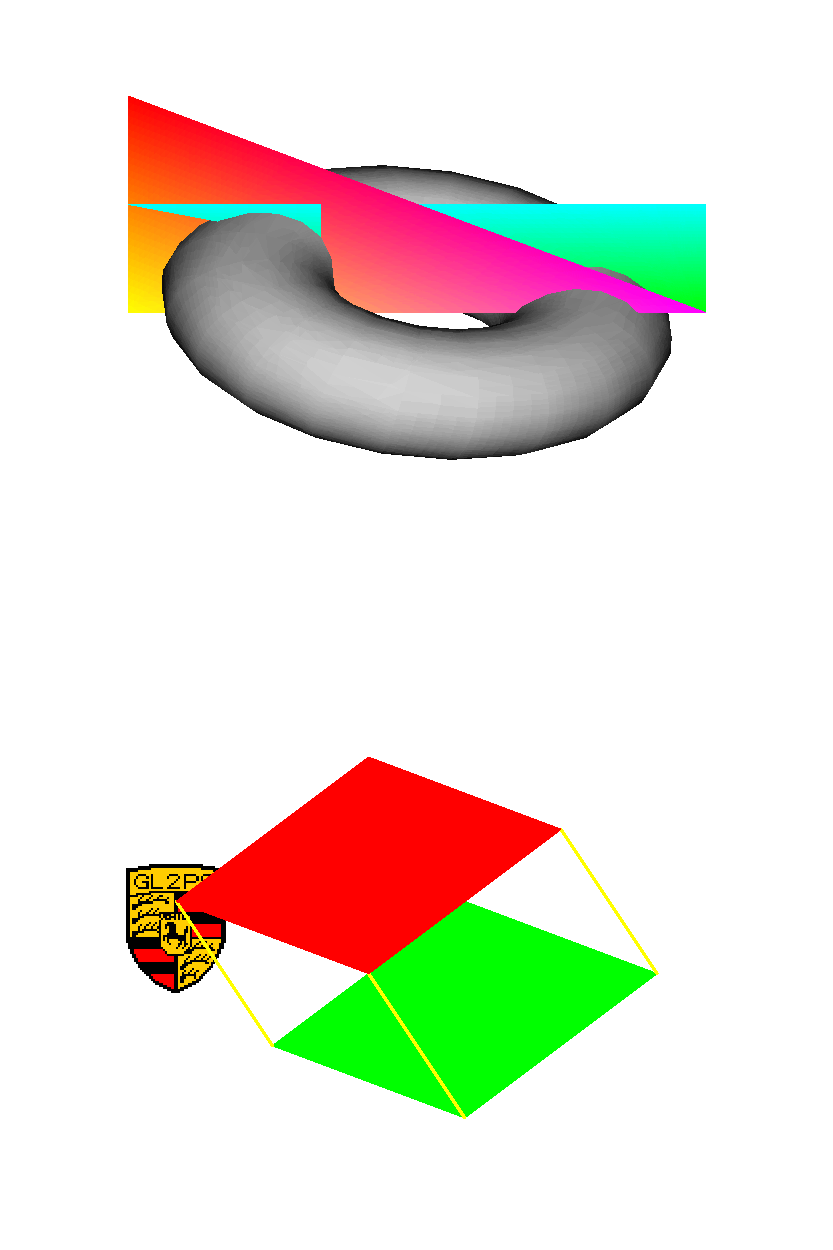
\includegraphics{outLatex}
\end{picture}%
\begin{picture}(400,600)(0,0)
\put(26.9229,389.769){\makebox(0,0)[lb]{Press:}}
\put(26.9229,376.269){\makebox(0,0)[lb]{  s: to save the images}}
\put(26.9229,362.769){\makebox(0,0)[lb]{  t: to alternate between teapot and torus}}
\put(26.9229,349.269){\makebox(0,0)[lb]{  v: to alternate between single and multiple viewport modes}}
\put(26.9229,335.769){\makebox(0,0)[lb]{  q: to quit}}
\put(26.9229,322.269){\makebox(0,0)[lb]{Click and move the mouse to rotate the objects}}
\end{picture}
}
%\caption{Sample output of the test program}
%\end{figure}

\section{Tips and tricks}
\label{sec:tips}

Here are, in no particular order, some useful tips and solutions to common
problems:
\begin{itemize}
\item For PDF (both compressed and non-compressed) and for compressed
  PostScript and SVG output, files should always be opened in binary
  mode, i.e., with \dd{fopen(..., "wb")}, instead of \dd{fopen(...,
    "w")}.
\item Blending is not yet very well supported by many viewers/printers. To
  disable blending entirely, add \dd{GL2PS_NO_BLENDING} to the list of
  options passed to \dd{gl2psBeginPage}.
\item Make sure that localization is turned off when using GL2PS, via:
\begin{verbatim}
  unsigned char *oldlocale = setlocale(LC_NUMERIC, "C");

  /* gl2ps drawing stuff */

  setlocale(LC_NUMERIC, oldlocale);
\end{verbatim}
  French or German localizations would for example lead to corrupted output
  files, as they represent the decimal point by a comma.
\item If you plan to convert PostScript files into PDF files, you may need
  to disable the use of the Level 3 PostScript \dd{shfill} operator, i.e.,
  add \dd{GL2PS_NO_PS3_SHADING} to the list of options passed to
  \dd{gl2psBeginPage}. (Note that you can also edit the output file \emph{a
    posteriori}---just set \dd{/tryPS3shading} to \dd{false} in the
  PostScript file header.) The best way to generate PDF files is of course
  to set the \dd{format} argument to \dd{GL2PS_PDF} in the
  \dd{gl2psBeginPage} call...
\item By default, GL2PS checks if blending is globally enabled in
  \dd{gl2psBeginPage()}. To enable blending for selected primitives
  only, you should use \dd{gl2psEnable(GL2PS_BLEND)} and
  \dd{gl2psDisable(GL2PS_BLEND)} pairs around the OpenGL calls that
  need blending. (Warning: this might change in future releases.)
\item \dd{gl2psEnable(GL2PS_LINE_STIPPLE)} uses the current values of
  the OpenGL stippling options to compute the stippling pattern and
  repetition factor. You thus need to call
  \dd{gl2psEnable(GL2PS_LINE_STIPPLE)} \emph{after} calling
  \dd{glLineStipple(factor, pattern)}.
 \end{itemize}

\section{Limitations}
\label{sec:limitations}

GL2PS works by capturing the contents of the OpenGL feedback
buffer\footnote{See the description of \dd{glFeedbackBuffer} and
\dd{glRenderMode(GL_FEEDBACK)} in the OpenGL documentation.}. As such, all
the OpenGL operations applied in the pipeline after the creation of the
feedback buffer will be ignored or have to be duplicated by GL2PS (e.g.\
font/image rendering, polygon offset or line stippling---see
sections~\ref{sec:gl2psText}, \ref{sec:gl2psDrawPixels},
\ref{sec:gl2psEnable} and \ref{sec:gl2psPointSize}).

Other limitations include:
\begin{itemize}
\item
Rendering large and/or complicated scenes is slow and/or can lead to large
output files. This is normal: vector-based images are not destined to
replace bitmap images. They just offer an alternative when high quality
(especially for 2D and small 3D plots) and ease of manipulation (how do you
change the scale, the labels or the colors in a bitmap picture long after
the picture was produced, and without altering its quality?) are important.
\item
Transparency is only supported for PDF and SVG output.
\item
GL2PS does not support textures, fog effects, etc.
\end{itemize}

% Other implementation Notes:
%
% OpenGL feedback buffer
% describe Simple depth sort
%          3D BSP tree
%          2D BSP image tree for occlusion culling
% float vs. double
% polygon offsets
% PostScript shading
%
% From the GLpr FAQ:
%
% 3. Can GLpr handle 2D texture mapping?
%
%    Only for pixel-based output (i.e., captured with glpImage()).  GLpr
%    cannot duplicate the effects of texture mapping for vector
%    (move-draw) output.  Unfortunately, the information required is not
%    present in the OpenGL feedback buffer.
%
% 4. Can GLpr handle 1D texture mapping?
%
%    Not in the present release.  However, future releases may provide
%    support for 1D texture maps (e.g.\ color lookup).
%
% Add references:
% - Fuchs, Kedem and Naylor for the BSP
% - Kilgard+OpenGL spec for the feedback buffer

\section{Contributors}
\label{sec:contrib}

\noemail{Michael Sweet}{mike@easysw.com} for the original implementation of
the feedback buffer parser;
%
\noemail{Bruce Naylor}{naylor@comp-graphics.com} for BSP tree and occlusion
culling hints;
%
\noemail{Marc Um{\'e}}{marc.ume@digitalgraphics.be} for the original list
code;
%
\noemail{Jean-Fran\c{c}ois Remacle}{remacle@gce.ucl.ac.be} for plane equation
fixes;
%
\noemail{Bart Kaptein}{B.L.Kaptein@lumc.nl} for memory leak fixes;
%
\noemail{Quy Nguyen-Dai}{quy@nguyendai.org} for output file size optimization;
%
\noemail{Sam Buss}{sbuss@ucsd.edu} for the \dd{shfill}-based smooth shaded
triangle code;
%
\noemail{Shane Hill}{Shane.Hill@dsto.defence.gov.au} for the landscape option
implementation;
%
\noemail{Romain Boman}{r_boman@yahoo.fr} for the Windows dll generation;
%
\noemail{Diego Santa Cruz}{Diego.SantaCruz@epfl.ch} for the new optimized
shaded triangle code and the \dd{shfill} management;
%
\noemail{Shahzad Muzaffar}{Shahzad.Muzaffar@cern.ch} and \noemail{Lassi
Tuura}{lassi.tuura@cern.ch} for the new occlusion culling code, the
improvement of \dd{GL2PS_BEST_ROOT} and the imagemap support;
%
\noemail{Guy Barrand}{barrand@lal.in2p3.fr} for his work on
\dd{gl2psDrawPixels} and the new viewport management;
%
\noemail{Rouben Rostamian}{rostamian@umbc.edu} and \noemail{Prabhu
Ramachandran}{prabhu@aero.iitm.ernet.in} for various bug reports and fixes;
%
\noemail{Micha Bieber}{bieber@traits.de} for the PDF code;
%
\noemail{Olivier Couet}{couet@mail.cern.ch} for the initial SVG code;
%
\noemail{Fabian Wenzel}{wenzel@tu-harburg.de} for the PGF code and the
backend reorganization;
%
\noemail{Shai Ayal}{shaiay@gmail.com} for rotated text support in
PostScript;
%
\noemail{Ian D. Gay}{gay@sfu.ca} for 64 bit arch patch;
%
\noemail{Cosmin Truta}{cosmin@cs.toronto.edu} and \noemail{Baiju
  Devani}{b.devani@gmail.com} for various bug fixes and the new
\dd{gl2psSpecial} code;
%
\noemail{Alexander Danilov}{danilov@lanl.gov} for a polygon offset bug
fix;
%
\noemail{Ben Fletcher}{ben.fletcher@dsto.defence.gov.au} for a
stippling pattern parser bug report;
%
\noemail{Jason Anderssen}{janderssen@exactal.com} for memory leak fix
in pdf code;
%
\noemail{Sylvestre Ledru}{sylvestre.ledru@scilab.org} for SVG patches;
%
\noemail{Calixte Denizet}{Calixte.Denizet@ac-rennes.fr} for 64 bit patch;
%
\noemail{Ion Vasilief}{lion\_vasilief@yahoo.fr} and Paul Griffiths for
rotated text in PDF output;
%
\noemail{Ben Abbott}{bpabbott@mac.com} for text alignment in SVG.

\section{Links}
\label{sec:links}

\dd{GL2PS} was inspired by Mark Kilgard's original ``rendereps'' tutorial
(\url{http://www.opengl.org/resources/code/samples/mjktips/Feedback.html})
and Michael Sweet's GLP library (\url{http://www.easysw.com/~mike/opengl/}).
The (commercial) GLpr library from CEI (\url{http://www.ceintl.com/}) used
to provide functionality similar to GL2PS but does not seem to be available
anymore.

%\noemail{Toby White}{tow@sdf.lonestar.org} maintains a Python wrapper for
%\dd{GL2PS}, available at \url{http://tow.freeshell.org/software.html}.

\section{Versions}

\begin{description}
\item[0.1] (Feb 12, 2000) First distributed version.
\item[0.2] (Feb 20, 2000) Added \dd{GL2PS_POLYGON_BOUNDARY} and
  \dd{GL2PS_BEST_ROOT}. API change: changed arguments of \dd{gl2psBeginPage}
  and \dd{gl2psText}. Corrected some memory allocation stuff. First version
  of this user's guide.
\item[0.21] (Mar 16, 2000) Initialization fixes.
\item[0.3] (Jul 29, 2000) Code cleanup. Added \dd{GL2PS_LINE_STIPPLE}.
\item[0.31] (Aug 14, 2000) Better handling of erroneous primitives.
\item[0.32] (May 23, 2001) Fixed memory leaks.
\item[0.4] (Jun 12, 2001) Added \dd{gl2psPointSize} and
  \dd{gl2psLineWidth}. Some code cleanup to allow easier generation of
  vector file formats other than postscript.
\item[0.41] (Aug 6, 2001) Fixed string allocation (1 char too short). Set
  smaller default line width.
\item[0.42] (Oct 8, 2001) Optimization of output file size. PostScript
  header cleanup. Better line width computation.
\item[0.5] (Nov 19, 2001) API change: new \dd{format} and \dd{filename}
  arguments for \dd{gl2psBeginPage}. Better PostScript handling of smooth
  shaded primitives. Fix handling of zero-length strings. New options for
  \LaTeX\ output. Changed (again) the line width computation.
\item[0.51] (Jan 22, 2002) Fixed erroneous drawing of text primitives lying
  outside the viewport.
\item[0.52] (Feb 14, 2002) New \dd{GL2PS_LANDSCAPE} option.
\item[0.53] (Mar 11, 2002) New \dd{GL2PSDLL} compilation flag to allow the
  generation of a Windows dll.
\item[0.6] (Jun 4, 2002) Fixed some incoherences in string allocation; fixed
  sorting of text objects; removed (non functional) occlusion culling code;
  fixed handling of color and line width attributes when gl2ps was called
  multiple times inside the same program.
\item[0.61] (Jun 21, 2002) Fixed the fix for the sorting of text objects;
  introduced tolerance for floating point comparisons.
\item[0.62] (Sep 6, 2002) New \dd{GL2PS_EPS} option to produce Encapsulated
  PostScript files; optimized drawing of shaded primitives; new
  \dd{GL2PS_NO_PS3_SHADING} option and \dd{gl2psNumShadeColors} function to
  control the use of the PostScript level 3 \dd{shfill} operator (usually
  not well handled when converting to PDF).
\item[0.63] (Nov 12, 2002) Changed \dd{GLvoid} to \dd{void} to accommodate
  some SUN compilers; made subdivision parameters modifiable a posteriori in
  the output file; revised documentation.
\item[0.7] (Dec 11, 2002) Occlusion culling (\dd{GL2PS_OCCLUSION_CULL}) is
  (finally!) working thanks to the great work of Shahzad Muzaffar; enhanced
  \dd{GL2PS_BEST_ROOT}.
\item[0.71] (Dec 13, 2002) Removed C++ style comments inadvertently left in
  the code; added example program \dd{gl2psTest.c} to the distribution.
\item[0.72] (Jan 21, 2003) Fixed crash in occlusion culling code; enhanced
  documentation.
\item[0.73] (Jan 30, 2003) Minor code cleanup.
\item[0.8] (Mar 10, 2003) API change: \dd{gl2psNumShadeColors} has been
  removed and the color subdivision parameters \dd{nr}, \dd{ng} and \dd{nb}
  are now given as arguments to \dd{gl2psBeginPage}; API change:
  \dd{gl2psBeginPage} takes an additional argument (\dd{viewport}) to
  specify the print viewport; new \dd{gl2psDrawPixels} interface to produce
  mixed mode (vector+raster) PostScript output; new \dd{gl2psBeginViewport}
  and \dd{gl2psEndViewport} interface to handle multiple OpenGL viewports;
  fixed small bug in occlusion culling code; better error handling.
\item[0.81] (Mar 22, 2003) Fixed small typos in comments and documentation.
\item[0.9.0] (Jun 2, 2003) Fixed smooth shading detection for mixed
  smooth/flat shaded scenes; new library numbering scheme
  (``major.minor.patch'').
\item[0.9.1] (Jun 12, 2003) Fixed two \dd{GL2PS_TEX} output bugs
  (\dd{glRenderMode} not reset to \dd{GL_RENDER} + crash when printing empty
  scenes); changed default pixmap depth to 8 bits per color component;
  changed default line cap to ``Butt cap'' and default line join to ``Miter
  join''.
\item[0.9.2] (Jul 4, 2003) Improved occlusion culling; new
  \dd{GL2PS_USE_CURRENT_VIEWPORT} option.
\item[1.0.0] (Sep 24, 2003) Native PDF support contributed by Micha
  Bieber.
\item[1.1.0] (Nov 4, 2003) New \dd{GL2PS_COMPRESS} option to create
  compressed PostScript and PDF files; fixed small bug in the PDF
  output that prevented the PDF files to be correctly included in
  \LaTeX\ documents; new alternative license (see \dd{COPYING.GL2PS}).
\item[1.1.1] (Nov 9, 2003) Small memory optimization; documentation update
  (binary files, fonts).
\item[1.1.2] (Nov 16, 2003) Fixed various compiler warnings (mostly
  for Windows Visual C++).
\item[1.2.0] (May 13, 2004) New (experimental...) transparency support for
  PDF output; fixed bug for empty feedback buffer but non-empty primitive
  list; fixed more compiler warnings and cleaned up the code (mostly to
  reduce the global namespace pollution).
\item[1.2.1] (Jul 13, 2004) New imagemap support for PostScript output; new
 text alignment support for PostScript and \LaTeX\ output; new support for
 rotated text for \LaTeX\ output; fixed NULL check on input strings in
 \dd{gl2psBeginPage}.
\item[1.2.2] (Sep 21, 2004) Fixed a couple of small bugs in the example
  code.
\item[1.2.3] (Dec 23, 2004) Fixed small bugs in (unused) PostScript pixmap
  code; better scaling of the z-buffer (improves
  \dd{GL2PS_SIMPLE_LINE_OFFSET} and occlusion culling); added support
  for general stippling patterns.
\item[1.2.4] (Apr 27, 2005) Fixed feedback buffer test for
  \dd{GL2PS_TEX} output; fixed missing brace in \LaTeX\ output for
  text aligned using \dd{GL2PS_TEXT_C}; fixed clipping in
  multi-viewport PostScript output when \dd{GL2PS_DRAW_BACKGROUND} is
  not set; new \dd{gl2psSetOptions} interface to change the current
  options on the fly.
\item[1.2.5] (Jun 18, 2005) Fixed a couple of uninitialized variables in
  PDF code; new \dd{GL2PS_TIGHT_BOUNDING_BOX} option; added rotated
  text support for PostScript output.
\item[1.2.6] (Jun 22, 2005) Fixed crash when creating PDF file with
  overflowing feedback buffer (bug introduced in 1.2.5); added
  additional example program \dd{gl2psTestSimple.c} to the
  distribution.
\item[1.2.7] (Feb 15, 2006) Fixed bug that could cause sorting to be
  inverted in BSP mode (bug introduced in 1.2.3); added limited
  support for SVG and PGF formats; made backend code more generic.
\item[1.3.0] (Aug 8, 2006) Full SVG support; improved line stippling
  (whenever possible lines are now rendered in a single path); better
  sorting of text and bitmap elements; new function \dd{gl2psSpecial}
  to print device-specific strings in the output stream.
\item[1.3.1] (Aug 11, 2006) Fixed a small bug for multi-viewport
  PostScript output, where a viewport could be drawn with an unwanted
  colored outline.
\item[1.3.2] (Nov 5, 2006) Fixed bug in polygon offset computation;
  fixed landscape mode in SVG; fixed potential out-of-bounds array
  access in stippling pattern parser.
\item[1.3.3] (Feb 28, 2009) Fixed memory leak in PDF code; added
  \dd{gl2psGetOptions}; nicer SVG rendering (crispEdges, font attributes);
  fixed possible divisions by zero.
\item[1.3.4] (Sep 30, 2009) Added support for rotated text in SVG output;
  fixed MSVC warnings.
\item[1.3.5] (Oct 16, 2009) Added support for rotated text in PDF output;
  fixed PDF image output when compiled in 64 bit mode; added cmake
  configuration.
\item[?] (?) Added support for PixelZoom (set using glPixelZoom) in
  postscript images; fixed text rotation in TeX; added support for text
  alignment in SVG; fixed other minor bugs.
\end{description}

\special{html:<p>
  <form action="https://www.paypal.com/cgi-bin/webscr" method="post">
  <input type="hidden" name="cmd" value="_xclick">
  <input type="hidden" name="business" value="geuzaine@acm.caltech.edu">
  <input type="hidden" name="item_name" value="GL2PS donation">
  <input type="hidden" name="no_note" value="1">
  <input type="hidden" name="currency_code" value="USD">
  <input type="hidden" name="tax" value="0">
  <input type="image" src="/images/donation.gif" name="submit"
         alt="Make a donation with PayPal">
  </form>
  <p>Back to <a href="/">geuz.org</a>}

\end{document}
